\documentclass[a4paper,12pt]{article}
\usepackage[T1]{fontenc}
\usepackage{fullpage,graphicx,psfrag,amsmath,amsfonts}
\usepackage[small,bf]{caption}
\usepackage[utf8]{inputenc}
\usepackage[english]{babel}
\usepackage{lipsum}
\usepackage{url}
\usepackage{fancyvrb}
\usepackage{bm}
\usepackage{float}
% \usepackage{mathptmx}
\usepackage[p,osf]{cochineal}
\usepackage{listings}
\usepackage[varqu,varl,var0]{inconsolata}
\usepackage[scale=.95,type1]{cabin}
\usepackage[cochineal,vvarbb]{newtxmath}
\usepackage[cal=boondoxo]{mathalfa}
\usepackage{enumitem}
\setitemize{noitemsep,topsep=0pt,parsep=0pt,partopsep=0pt}
\begin{document}
\author{Filippo Grotto VR460638}

\title{Fetal Health Classification  \\[1ex] \large Machine Learning and Artificial Intelligence \\[1ex] \large Academic year 2020/2021}

\maketitle
\newpage
\tableofcontents
\newpage

\section{Motivation and rationale}
This project is heavily inspired by a kaggle task \cite{kaggle} about fetal health classification.
\begin{quote}
Reduction of child mortality is reflected in several of the United Nations' Sustainable Development Goals and is a key indicator of human progress.
The UN expects that by 2030, countries end preventable deaths of newborns and children under 5 years of age, with all countries aiming to reduce under‑5 mortality to at least as low as 25 per 1,000 live births.

Parallel to notion of child mortality is of course maternal mortality, which accounts for 295 000 deaths during and following pregnancy and childbirth (as of 2017). The vast majority of these deaths (94\%) occurred in low-resource settings, and most could have been prevented.

In light of what was mentioned above, Cardiotocograms (CTGs) are a simple and cost accessible option to assess fetal health, allowing healthcare professionals to take action in order to prevent child and maternal mortality. The equipment itself works by sending ultrasound pulses and reading its response, thus shedding light on fetal heart rate (FHR), fetal movements, uterine contractions and more.
\end{quote}
In this context this project is not only an application of machine learning techniques but it also have a meaningful application into real world scenarios thanks to the real data provided.

\section{Brief State of Art}
The analysis of CTGs data is an important task in order to reduce maternal mortality. In particular, the literature is rich of several different machine learning techniques used to address the classification problem. For example K-NN and SVM has been extensively used to solve this type of task with successful results \cite{ml}. Moreover, in recent years, other techniques has proved to improve performances as reported in \cite{ann} using ANN (Artifical Neural Networks), using CNN (Convolutional Neural Network) \cite{cnn} and using XGBoost classifiers \cite{ml}. For the purpose of this project we will address classical machine learning techniques with a brief introduction to ANN. 

\section{Objective (Problem definition and Dataset)}
The dataset comes from UCI Machine Learning Repository \cite{uci} and it is composed by 
\begin{quote}
2126 fetal cardiotocograms (CTGs) automatically processed with the respective diagnostic features measured. The CTGs were classified by three expert obstetricians and a consensus classification label assigned to each of them. Classification was both with respect to a morphologic pattern (A, B, C. ...) and to a fetal state (N=normal; S=suspect; P=pathologic). Therefore the dataset can be used either for 10-class or 3-class experiments.
\end{quote}
We will address the 3-class classification problem so we will try to classify the data according to normal, suspect or pathologic.

\section{Methodology}
The classification problem is addressed using the following techniques:

\begin{itemize}
  \item Naive Bayes \cite{ml}
  \item SVM (with different kernels) \cite{ml}
  \item KNN (with different k based on preliminary analysis) \cite{ml}
  \item ANN \cite{ann}
\end{itemize}
Moreover, PCA and Fisher (LDA) dimensionality reduction techniques are considered as well as the effects of data scaling and/or normalization. Finally some exploration tasks are reported such as the use of a subset of features according to statistical correlation and a brief analysis of the semi-supervised problem.
\section{Experiments and Results}
\subsection{Dataset exploration}
The dataset is composed by 2126 entries with 22 features (21 features + fetal health which is our target for the classification). From a first analysis there are no null or empty values but there are 13 duplications which we dropped. A brief description of the dataset is reported in Fig \ref{fig:features}.

\begin{figure}[H]
\begin{center}
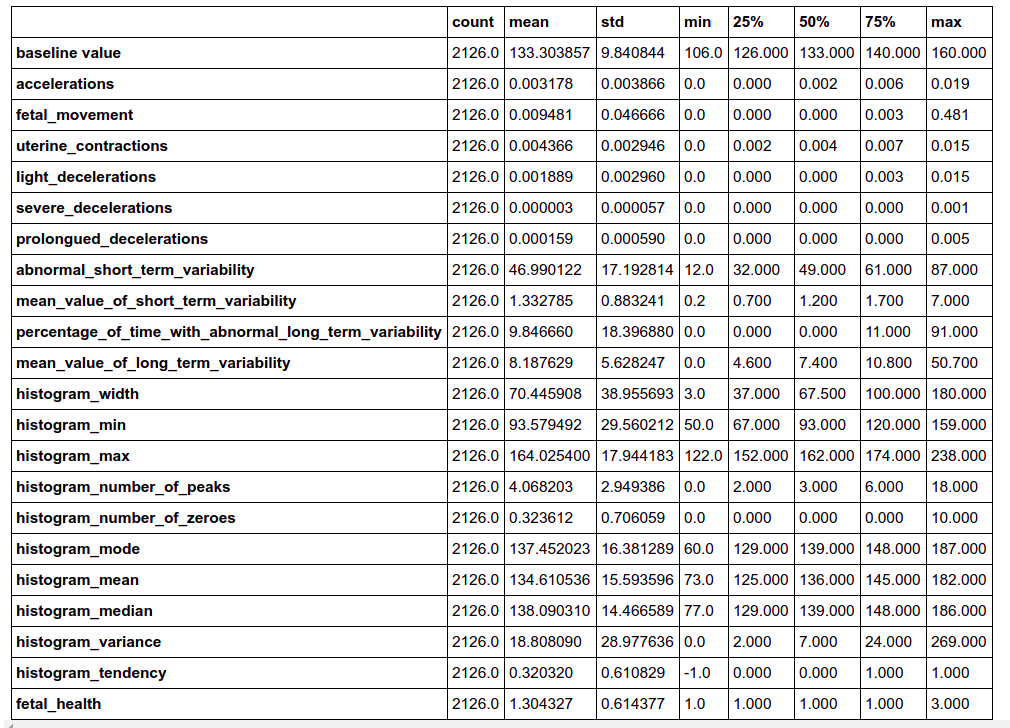
\includegraphics[width=1.0\textwidth]{images/features.png}
\end{center}
\caption{Description of all feature dataset}
\label{fig:features}
\end{figure}

\noindent Another observation to make is the presence of high class imbalance that comes from the real dataset. In Fig \ref{fig:imbalance} it is visible that \textbf{Normal} represents around the 78\% of the entire dataset.

\begin{figure}[H]
\begin{center}
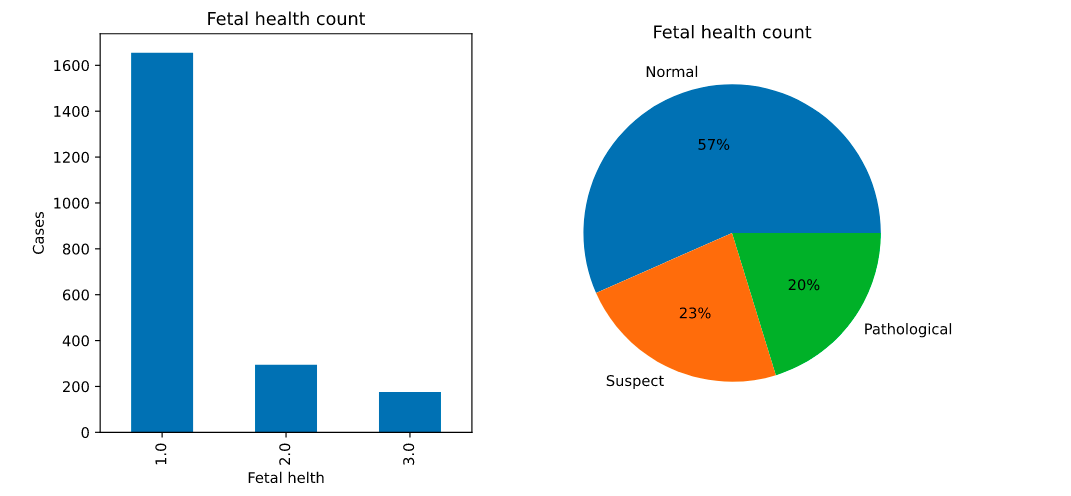
\includegraphics[width=1.0\textwidth]{images/imbalance.png}
\end{center}
\caption{Class imbalance in the dataset, around 78\% is classified as normal fetal health}
\label{fig:imbalance}
\end{figure}

\noindent Having verified the presence of class imbalance we will use different performance measures for our models in order to avoid misleading considerations:
\bigbreak
\begin{itemize}
  \item \textbf{Precision}
  \item \textbf{Accuracy} 
  \item \textbf{Recall}
  \item \textbf{F1 Score}
  \item \textbf{Confusion Matrix}
\end{itemize}

\bigbreak
\noindent
Moreover in order to deal with the class imbalance several options are possible:
\begin{itemize}
  \item Oversampling the dataset 
  \item Undersampling the dataset
  \item Use different weights in the classification
\end{itemize}
\bigbreak
\noindent In this context \textbf{oversampling} was evaluated as the best approach for this project since the dataset for the minority class is pretty limited and classifiers with different weights are not extremely performant for this scenario and it's difficult to estimate correct values of the weights (this comes from some preliminary tests).

\bigbreak
\noindent In Fig \ref{fig:hist} an histogram for each feature is provided. We could clearly see that at least 8 features are extremely skewed and contain a significant amount of outliers. In order to assure a flawless performance of the classifiers models we will scale every feature by standardization.

\begin{figure}[H]
  \begin{center}
  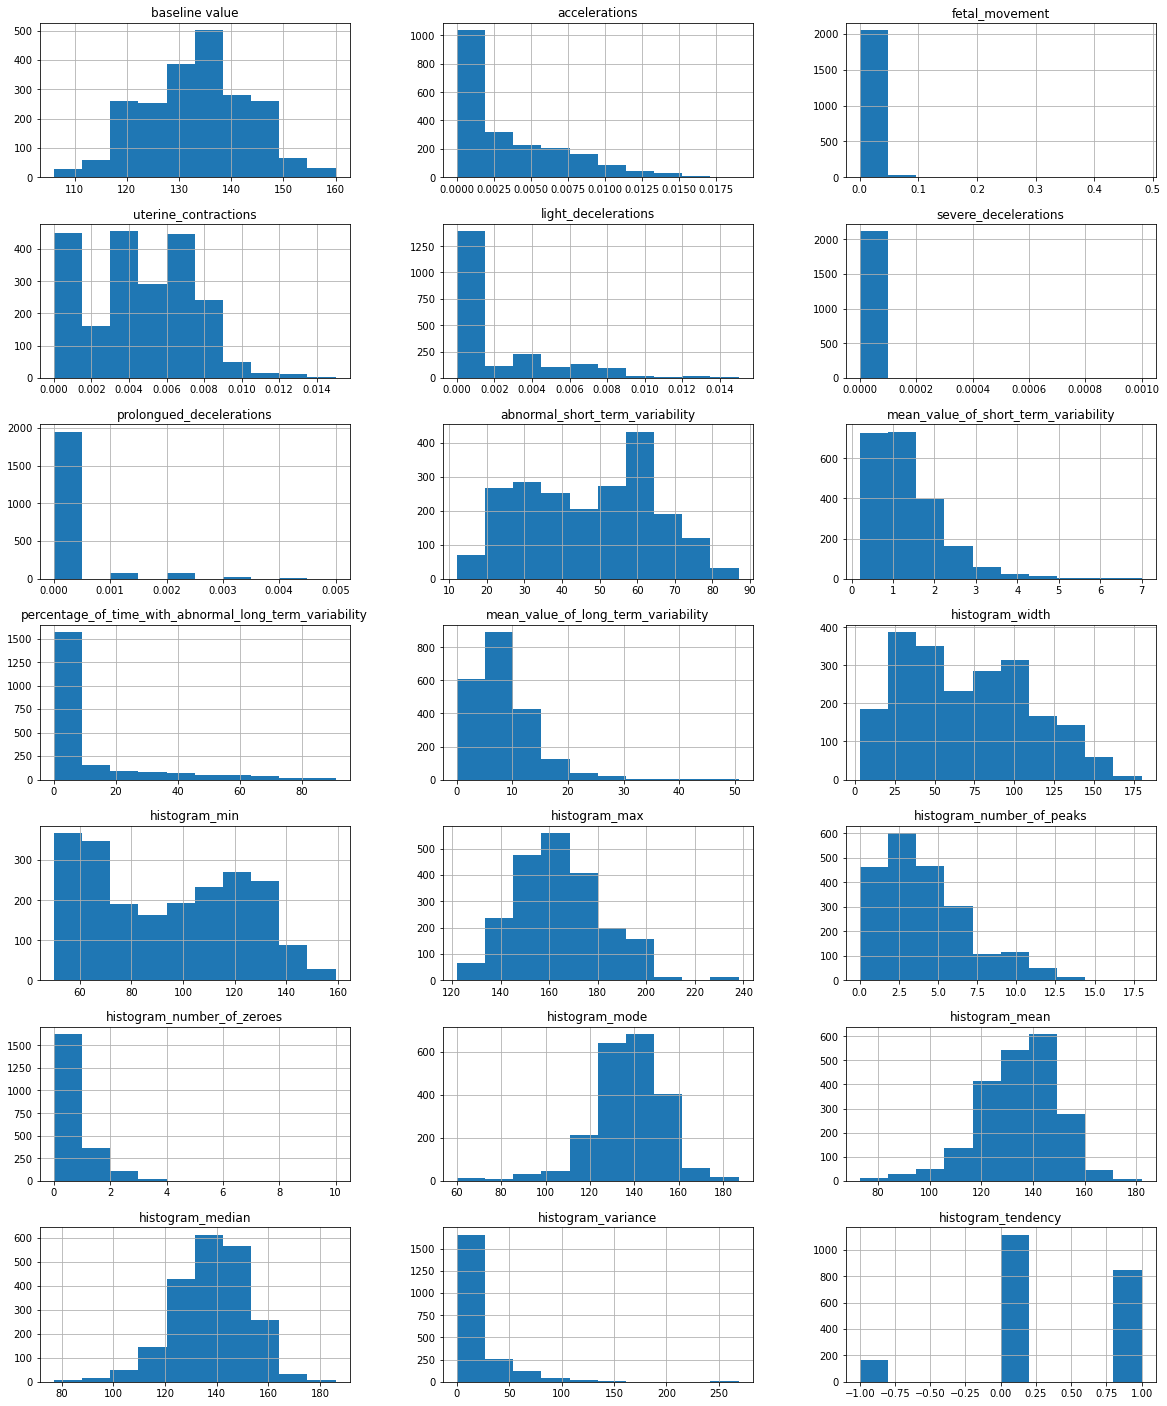
\includegraphics[width=1.0\textwidth]{images/hist.png}
  \end{center}
  \caption{Histogram of each feature}
  \label{fig:hist}
\end{figure}

\bigbreak
\noindent Finally we can analyse the correlation between features of the dataset in order to evaluate a possible subset to improve our performances. In table \ref{tab:correlation} the features with more than 30\% correlation with \textbf{fetal health} are reported.
In Fig \ref{fig:correlation} a heatmap is reported with the correlation between our features.

\begin{table}[H]
\begin{tabular}{ |p{10cm}||p{3cm}| }
  \hline
  Feature Name& Correlation \\
  \hline
  accelerations&                                            -0.364066\\
  prolongued decelerations&                                  0.484859\\
  abnormal short term variability&                           0.471191\\
  percentage of time with abnormal long term variability&    0.426146\\
  \hline
\end{tabular}
\caption{Feature with correlation higher than 30\%}
\label{tab:correlation}
\end{table}

\begin{figure}[H]
  \begin{center}
  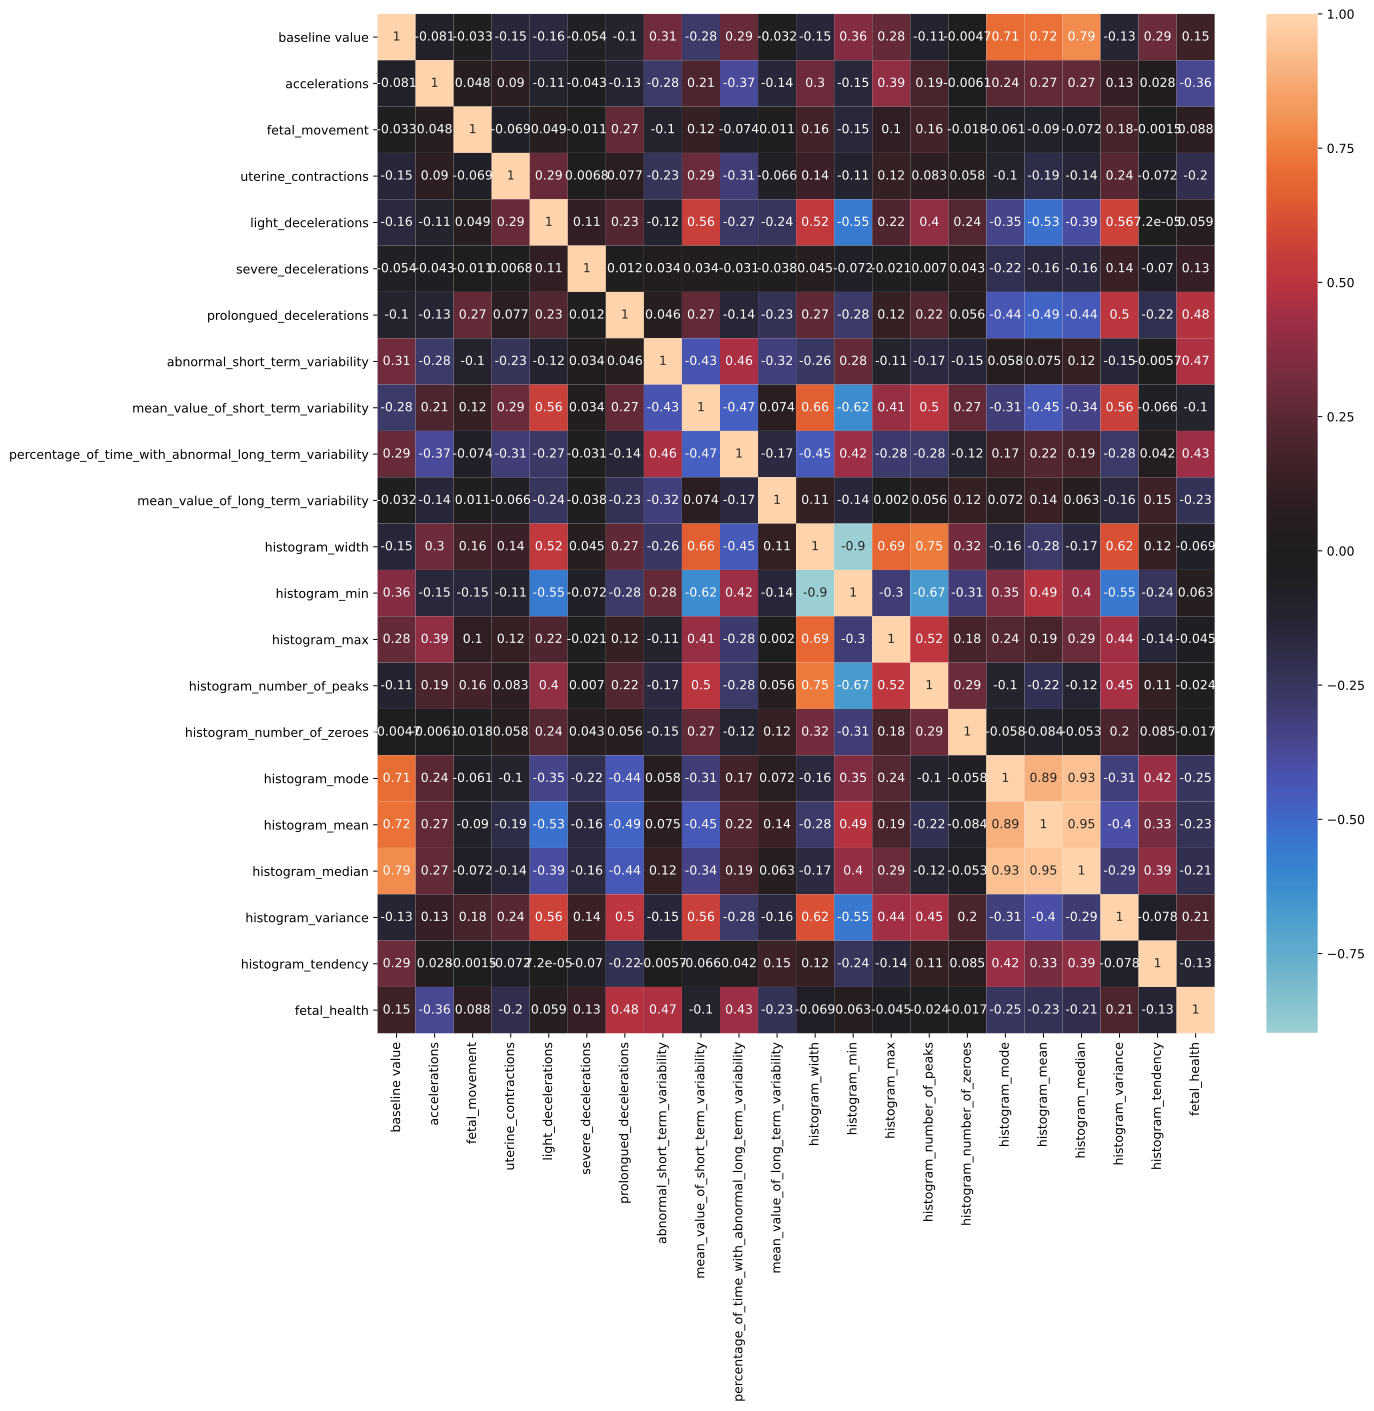
\includegraphics[width=0.9\textwidth]{images/correlation.png}
  \end{center}
  \caption{Correlation between features}
  \label{fig:correlation}
\end{figure}

\noindent As a result the features with high correlation are \textbf{accelerations}, \textbf{prolongued decelerations},\textbf{abnormal short term variability} and \textbf{percentage of time with abnormal long term variability}. They will be considered in a further analysis as a reasonable subset of the dataset to exploit our models.

\subsection{Data scaling}
In Fig \ref{fig:notscaled} the original data is reported. It's visible that the data requires a proper scaling to avoid the presence of dominant features that might affect our analysis. In Fig \ref{fig:scaled} the scaled data is reported where \textbf{StandardScaler} was used. Data normalization is not actually reported since from experiments it doesn't provide much more benefits and it's irrelevant for the sake of this report.

\begin{figure}[H]
  \begin{center}
  \includegraphics[width=0.7\textwidth]{images/not_scaledù.png}
  \end{center}
  \caption{Plot of the original data without scaling}
  \label{fig:notscaled}
\end{figure}
\begin{figure}[H]
  \begin{center}
  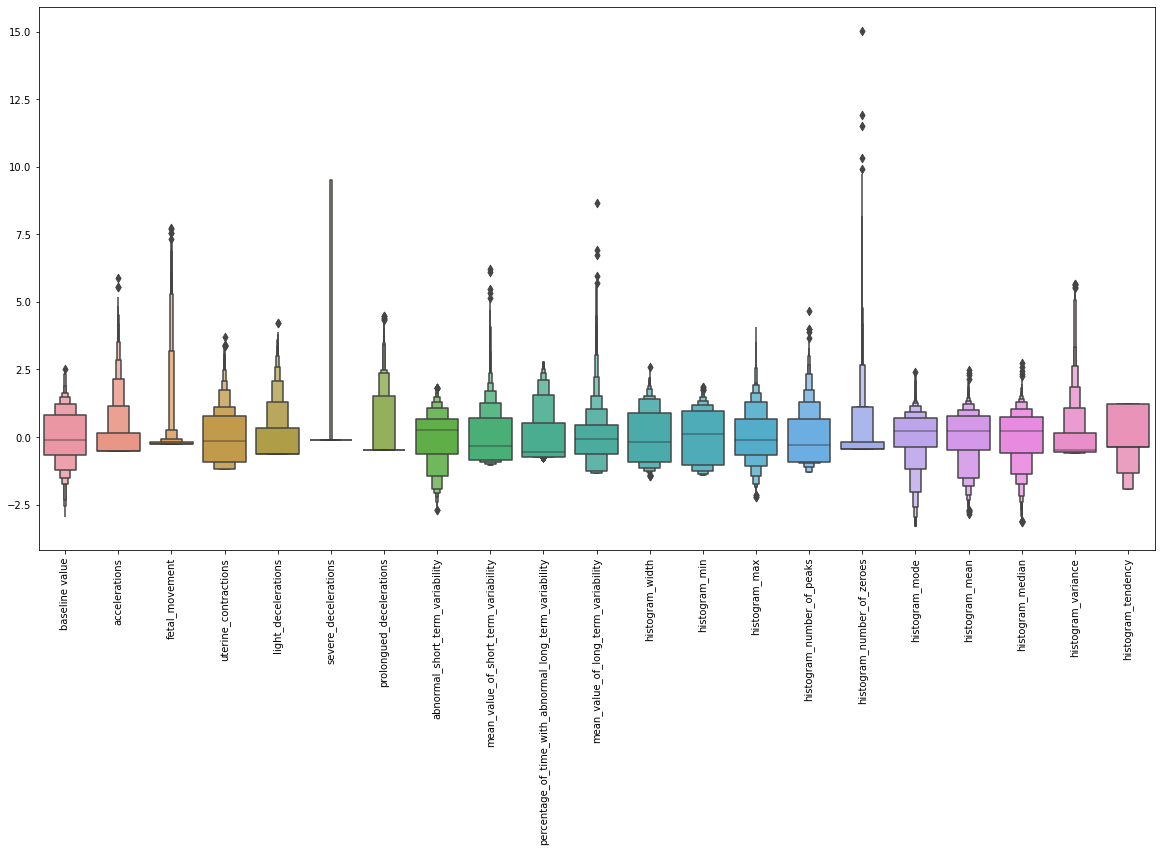
\includegraphics[width=0.7\textwidth]{images/scaled.png}
  \end{center}
  \caption{Plot of the scaled training set}
  \label{fig:scaled}
\end{figure}

\newpage
\subsection{PCA dimensionality reduction}
\bigbreak
\noindent In Fig \ref{fig:pca} the analysis of PCA dimensionality reduction is considered. In particular the graph rappresents the cumulative explained variation ratio with respect of all the possible components we might want to consider.

\begin{figure}[H]
  \begin{center}
  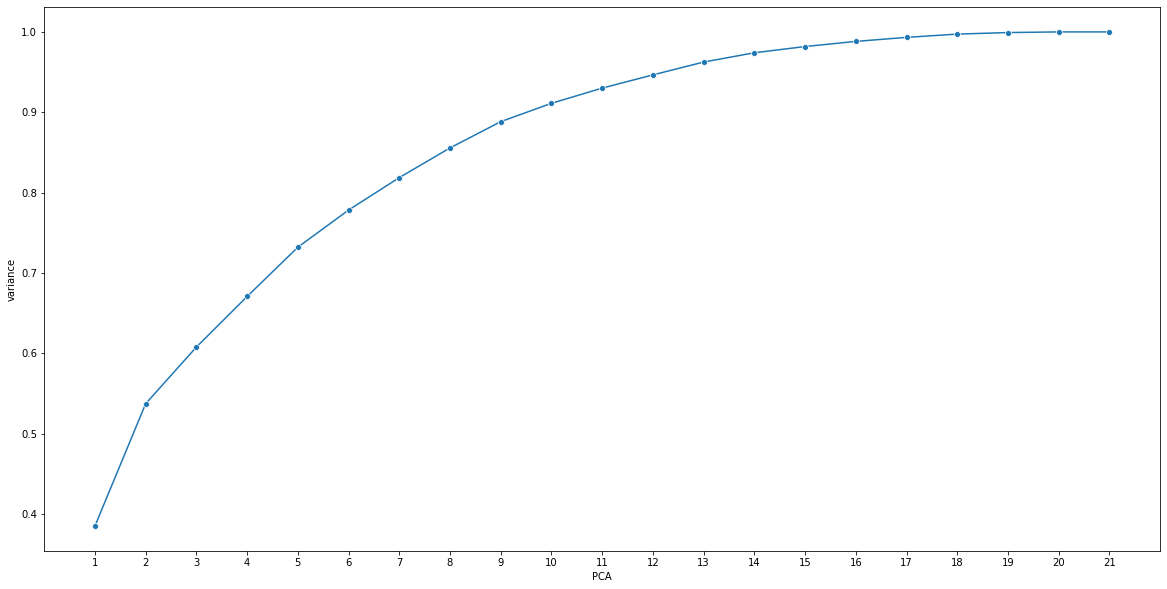
\includegraphics[width=1.0\textwidth]{images/pca.png}
  \end{center}
  \caption{PCA cumulative explained variance ratio wrt of components}
  \label{fig:pca}
\end{figure}

\noindent In particular the last five components don't provide much more information (close to zero) and with 6 components we have a representation of around 80\% of our dataset. In table \ref{tab:pca} the results obtained by our models over the 6 components are briefly reported to get an idea of the performances.

\begin{table}[H]
  \begin{tabular}{ |p{6cm}||p{2cm}|p{2cm}|p{2cm}|p{2cm}| }
    \hline
    Model& accuracy & precision  &  recall & f1 score \\
    \hline
    SVM linear           &0.813333&   0.821697&  0.813333&  0.814042\\
    SVM poly             &0.820000&   0.826573&  0.820000&  0.820346\\
    SVM rbf              &0.813333&   0.815441&  0.813333&  0.812814\\
    SVM sigmoid          &0.660000&   0.661235&  0.660000&  0.659368\\
    Gaussian NB          &0.753333&   0.774734&  0.753333&  0.756183\\
    \hline
  \end{tabular}
  \caption{Evaluation of our models over 6 PCA components}
  \label{tab:pca}
  \end{table}

\newpage
\subsection{LDA dimensionality reduction}

In this section a brief analysis of Linear Discriminant Analysis is reported in Fig \ref{fig:lda} where we can easily see that the cumulative variance ratio accumulated with 1 component rappresents around 80\% of our dataset.
Moreover, both the case with 1 and 2 components are briefly reported in table \ref{tab:lda1} and \ref{tab:lda2} to get an idea of the performances. 

\begin{figure}[H]
  \begin{center}
  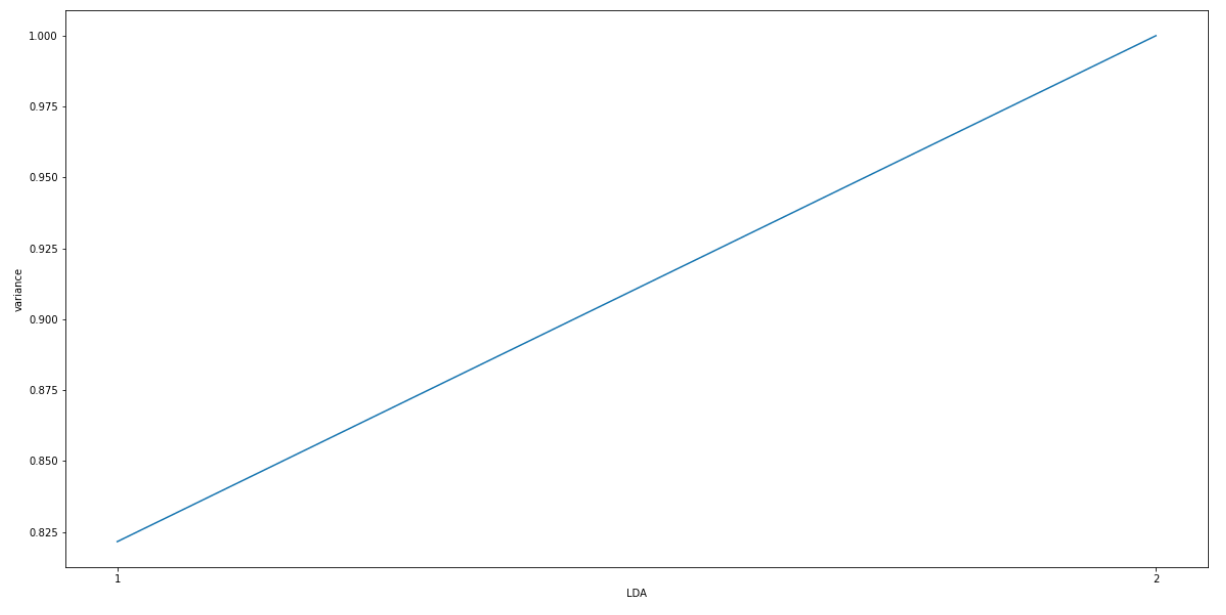
\includegraphics[width=0.8\textwidth]{images/lda.png}
  \end{center}
  \caption{LDA cumulative explained variance ratio wrt of components}
  \label{fig:lda}
\end{figure}


\begin{table}[H]
\begin{tabular}{ |p{6cm}||p{2cm}|p{2cm}|p{2cm}|p{2cm}| }
  \hline
  Model& accuracy & precision  &  recall & f1 score \\
  \hline
  SVM linear           &0.733333&   0.739409&  0.733333&  0.735703\\
  SVM poly             &0.740000&   0.782873&  0.740000&  0.747160\\
  SVM rbf              &0.766667&   0.788004&  0.766667&  0.771221\\
  SVM sigmoid          &0.560000&   0.548726&  0.560000&  0.552469\\
  Gaussian NB          &0.740000&   0.744999&  0.740000&  0.741770\\
  \hline
\end{tabular}
\caption{Evaluation of our models with 1 LDA component}
\label{tab:lda1}
\end{table}

\begin{table}[H]
\begin{tabular}{ |p{6cm}||p{2cm}|p{2cm}|p{2cm}|p{2cm}| }
  \hline
  Model& accuracy & precision  &  recall & f1 score \\
  \hline
  SVM linear           &0.800000&   0.810988&  0.800000&  0.801167\\
  SVM poly             &0.786667&   0.833078&  0.786667&  0.791542\\
  SVM rbf              &0.793333&   0.813034&  0.793333&  0.795674\\
  SVM sigmoid          &0.693333&   0.694028&  0.693333&  0.693031\\
  Gaussian NB          &0.793333&   0.815672&  0.793333&  0.796466\\
  \hline
\end{tabular}
\caption{Evaluation of our models with 2 LDA components}
\label{tab:lda2}
\end{table}


\noindent In general in case of uniformly distributed data, LDA almost always performs better than PCA. However if the data is highly skewed (irregularly distributed), like in our scenario, then it is advised to use PCA since LDA can be biased towards the majority class. \cite{pca-lda}. Finally, in this report the dimensionality reduction is actually not used since there are no benefits in having it as we will show in the following sections using all features for the classification task.

\newpage
\subsection{Model evaluations with the full dataset}

In this section the evaluations of several models are presented. The training dataset is oversampled using $SMOTE$ \cite{smote} and the test set is composed by 30\% of the minority class (50 samples) and the same amount of samples for the other two classes. In this way the testing dataset is balanced and the training dataset is oversampled for better training. This is a necessary step to deal with unbalanced classes and avoid metrics overestimations due to synthetic data in the testing set (the testing set must be real). 
The results of our models are reported in Fig \ref{fig:fulldataset}. It's visible that SVM with rbf kernel produces the best results over our dataset. This is coherent with the analysis in \cite{ml} and what the literature provides us about Support Vector Machines Kernels. All models use as default OneVsRest approach. Let's consider:
\begin{itemize}
  \item 1.0 Normal
  \item 2.0 Suspicious
  \item 3.0 Pathologic
\end{itemize}
\bigbreak
\begin{figure}[H]
  \begin{center}
  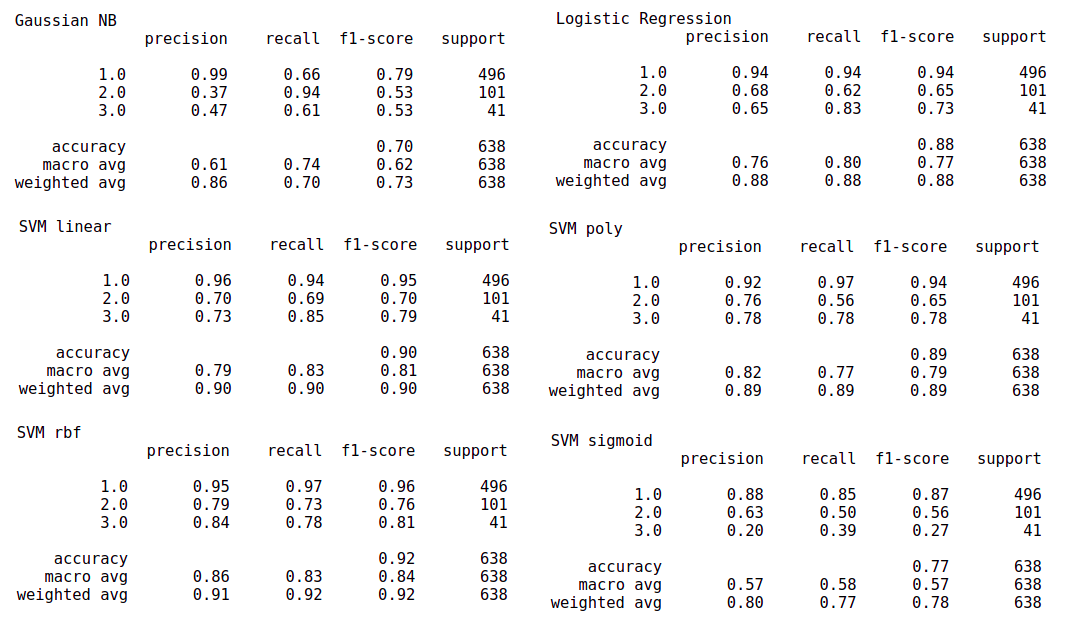
\includegraphics[width=1.0\textwidth]{images/fulldataset.png}
  \end{center}
  \caption{Results of the selected models over our dataset}
  \label{fig:fulldataset}
\end{figure}

\noindent From a brief analysis we can clearly see that SVM in general works pretty well over our dataset, Naive Bayes and SVM with sigmoid kernel are pretty bad in terms of precision for \textbf{suspicious} and \textbf{pathologic}. In general the class \textbf{Normal} has better performances. Moreover in Fig \ref{fig:confusion_svm} and Fig \ref{fig:confusion_bayes} the confusion matrixes for the svm with rbf kernel and Naive Bayes are respectively reported. What is clearly visible is the fact that for SVM with rbf there are few false positive and false negative values for the normal class which is a pretty good result but not perfect. For Naive Bayes we have a total of false negative values which is close to the true value which is pretty bad for our classification problem. In fact, in the real context, we can't accept to misclassify a suspicious element with a normal one but we can easily accept the opposite.

\begin{figure}[H]
  \begin{center}
  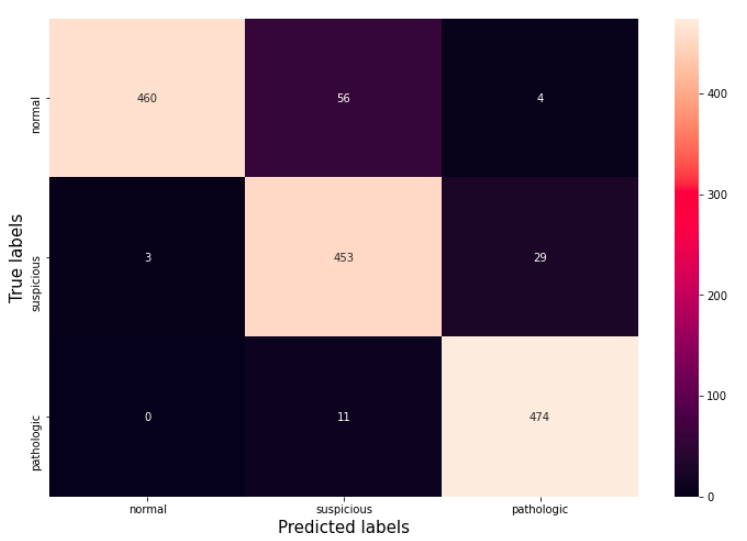
\includegraphics[width=0.8\textwidth]{images/svm_rbf.png}
  \end{center}
  \caption{Confusion matrix of SVM with rbf kernel}
  \label{fig:confusion_svm}
\end{figure}

\begin{figure}[H]
  \begin{center}
  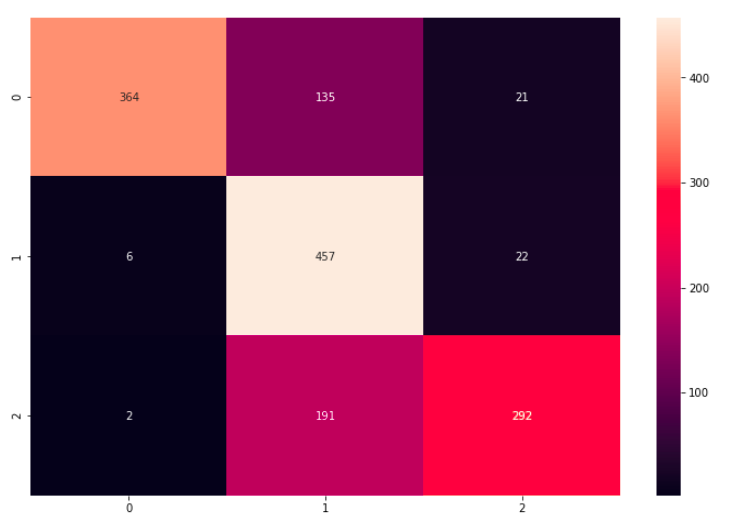
\includegraphics[width=0.8\textwidth]{images/confusion_naive.png}
  \end{center}
  \caption{Confusion matrix of Naive Bayes approach}
  \label{fig:confusion_bayes}
\end{figure}

\subsubsection{K-Nearest Neighbors}
In this section we will consider the use of K-NN (with an euclidean distance applied) to our dataset. In Fig \ref{fig:knn} a brief analysis of several k is provided with the related metrics to get an idea of which are the most promising values of K to use.

\begin{figure}[H]
  \begin{center}
  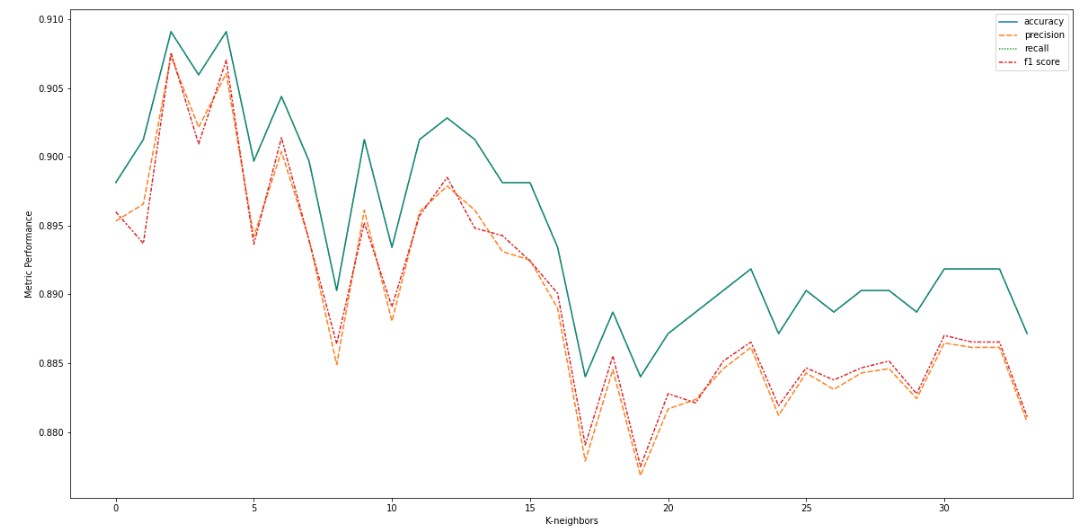
\includegraphics[width=1.0\textwidth]{images/knn.png}
  \end{center}
  \caption{K-NN metrics with respect of the value K-neighbors}
  \label{fig:knn}
\end{figure}

\noindent As a result the value K = 3 is the best choices. In Fig \ref{fig:knn2} the best case is considered and analysed.

\begin{figure}[H]
  \begin{center}
  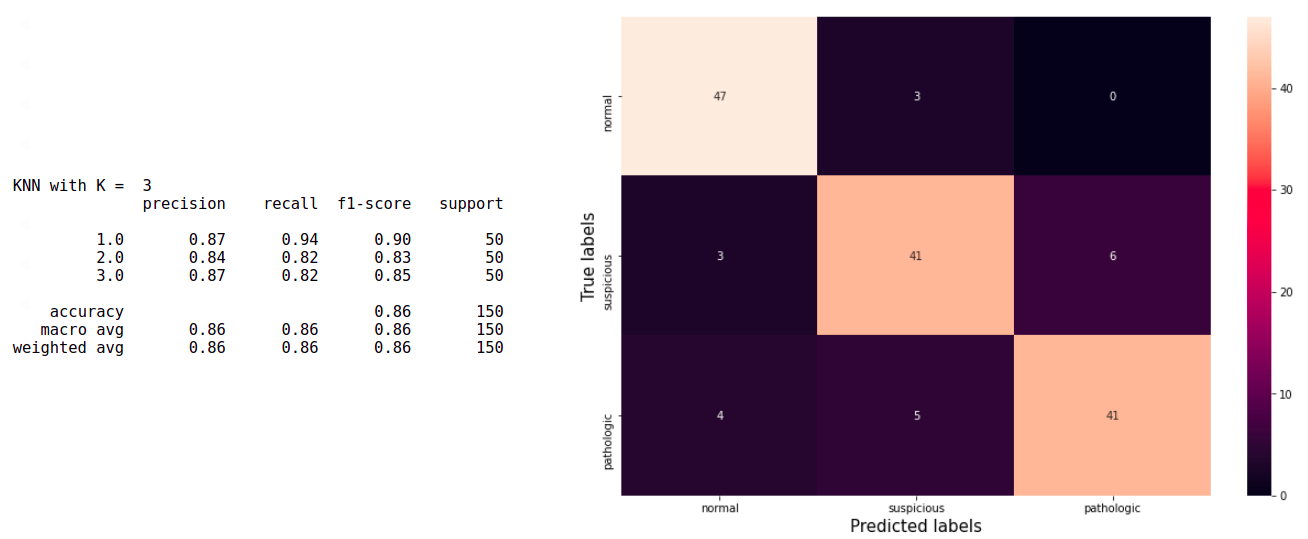
\includegraphics[width=0.9\textwidth]{images/knn2res.png}
  \end{center}
  \caption{K-NN with k=3 metrics and confusion matrix}
  \label{fig:knn2}
\end{figure}


\noindent As a conclusion K-NN with k=3 is a good model with few false positive for the normal class but we still find some difficulties for the two classes suspicious and pathologic due to the low amount of data available. Moreover the dataset is pretty limited so K-NN is suitable in this case but it might be extremely data intensive for large datasets.

\subsubsection{Artificial Neural Networks MLP}
In this section we will brief provide some results obtained by using Artificial Neural Networks to solve the classification problem. In particular we created a multilayer perceptron (MLP) with the following parameters
\begin{Verbatim}[fontsize=\small]
input_size = 21
hidden_size = 100
num_classes = 3
num_epochs = 100
batch_size = 50
learning_rate = 0.001
\end{Verbatim} 

\begin{Verbatim}[fontsize=\small]
# Fully connected neural network with one hidden layer
class NeuralNet(nn.Module):
  def __init__(self, input_size, hidden_size, num_classes):
      super(NeuralNet, self).__init__()
      self.fc1 = nn.Linear(input_size, hidden_size) 
      self.relu = nn.ReLU()
      self.fc2 = nn.Linear(hidden_size, num_classes)  
  
  def forward(self, x):
      out = self.fc1(x)
      out = self.relu(out)
      out = self.fc2(out)
      return out
\end{Verbatim}

\noindent The MLP uses one fully connected layer, a ReLU as activation function and another fully connected layer (Linear). The criterion used is CrossEntropyLoss. This model have an accuracy of around 85\% which makes it a good model for the classification task as reported in Fig \ref{fig:annres}.

\begin{figure}[H]
  \begin{center}
  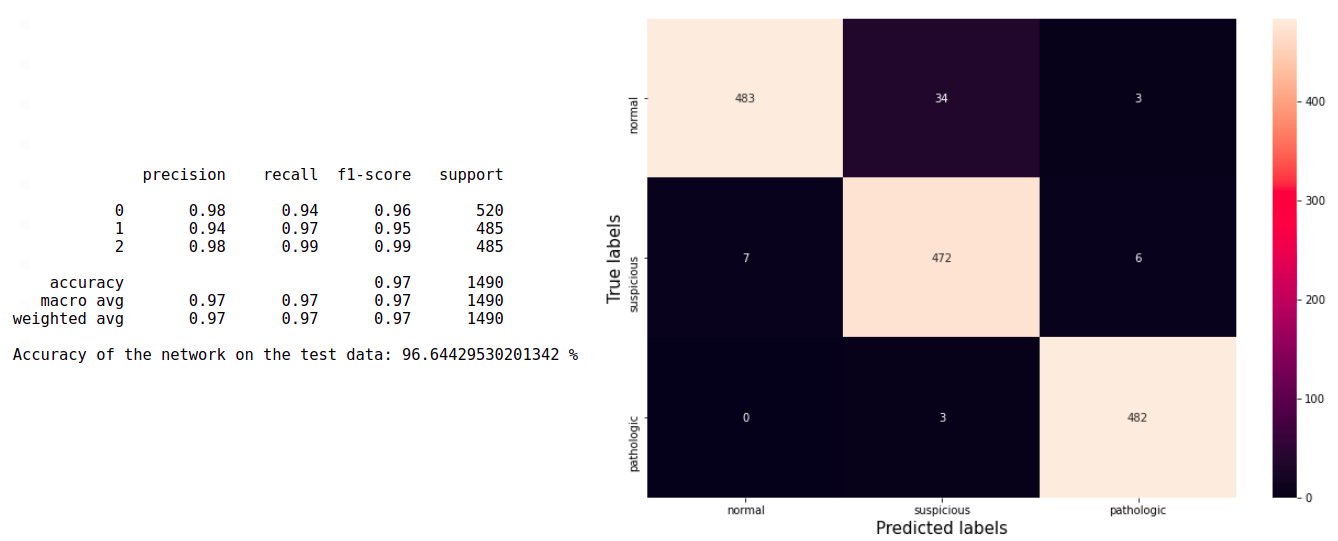
\includegraphics[width=1.0\textwidth]{images/ann_res.png}
  \end{center}
  \caption{Results of the MLP network}
  \label{fig:annres}
\end{figure}

\subsection{Other Exploratory Tasks}

\subsubsection{Models evaluation using a subset of features}

In this section an evaluation of our models over a subset of features defined in the previous section is presented. Only features with more than 30\% correlation with the target \textbf{fetal health} are used. They are reported in Table \ref{tab:correlation}. In Table \ref{tab:subset} the evaluations of our models are reported according to the defined metrics. Moreover, in Fig \ref{fig:poly} the classification report for the best model SVM rbf is reported.

\begin{table}[H]
\begin{tabular}{ |p{6cm}||p{2cm}|p{2cm}|p{2cm}|p{2cm}| }
  \hline
  Model& accuracy & precision  &  recall & f1 score \\
  \hline
  SVM linear &          0.76&   0.76&  0.76&  0.76\\
  SVM poly   &          0.81&   0.85&  0.81&  0.80\\
  SVM rbf    &          0.82&   0.82&  0.82&  0.82\\
  SVM sigmoid &         0.54&   0.53&  0.54&  0.51\\
  Gaussian Naive &         0.73&   0.76&  0.73&  0.73\\
  \hline
\end{tabular}
\caption{Evaluation of our models over a subset of features}
\label{tab:subset}
\end{table}

\begin{figure}[H]
  \begin{center}
  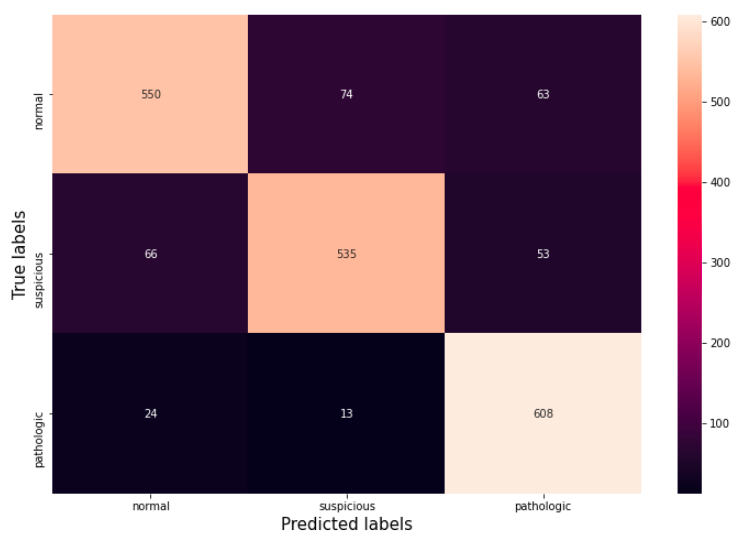
\includegraphics[width=0.8\textwidth]{images/svm_rbf_corr.png}
  \end{center}
  \caption{Detailed classification report for SVM with rbf kernel}
  \label{fig:poly}
\end{figure}

\noindent Not all the confusion matrixes are reported but both Gaussian Naive and SVM with sigmoid have severe problems in distinguish the two classes \textbf{Suspicious} and \textbf{Normal} since they report a lot of false positives and negatives. Anyway we showed how, using a lower number of features, we are still able to get pretty good results with a SVM with rbf and have a decent confusion matrix (low number of false positive and negative) even though it's not as good as using all the features. This is a reasonable result given the fact that the correlation was pretty low around 30\%.

\subsubsection{Semisupervised Problem}
In this section the semisupervised problem is briefly approached using a simple pseudo labelling method using the SVM rbf which proved to be one of the best classifier for this scenario. We use 100 samples per each class to build the labeled training dataset. We train the classifier with that labeled dataset (300,21) and then we predict the pseudo labels from the unlabeled part of the dataset (4515, 21). We combine the two results and we train a classifier using the full training dataset (with the true labels and the pseudo labels). Finally we predict the test dataset. The results for the semisupervised problem are reported in Fig \ref{fig:semi}, the results for the fully supervised problem are reported in Fig \ref{fig:fully}  

\begin{figure}[H]
  \begin{center}
  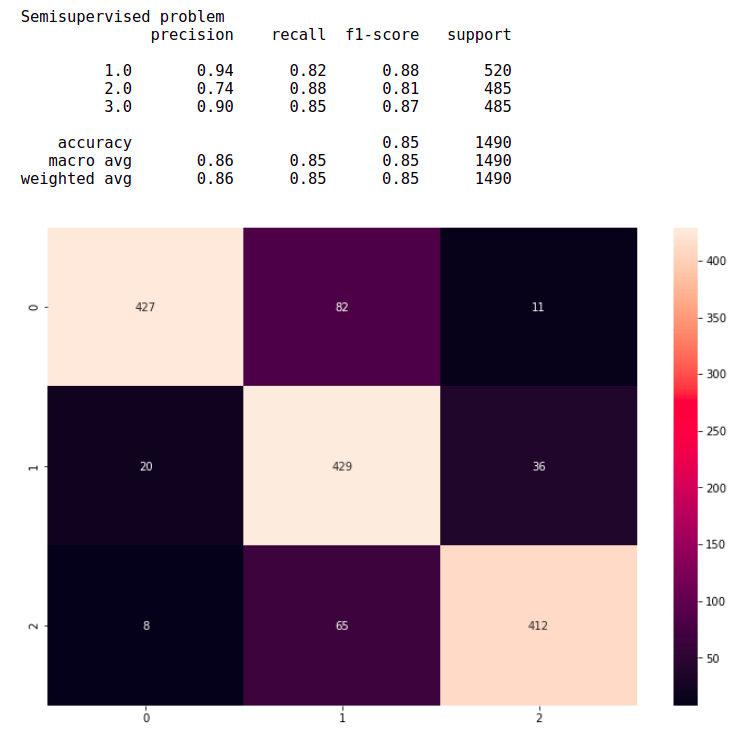
\includegraphics[width=0.8\textwidth]{images/semi.png}
  \end{center}
  \caption{Classification report for the semisupervised problem using OneVsOne SVM with rbf kernel}
  \label{fig:semi}
\end{figure}

\begin{figure}[H]
  \begin{center}
  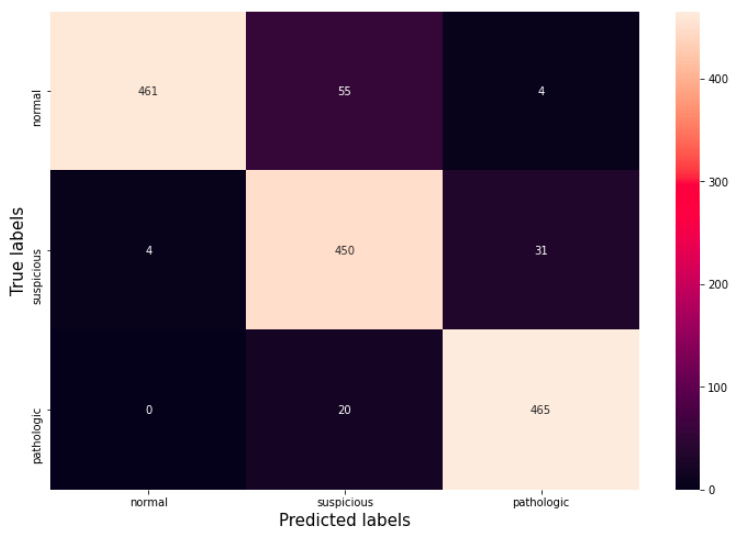
\includegraphics[width=0.8\textwidth]{images/fully.png}
  \end{center}
  \caption{Classification report for the fully supervised problem using OneVsOne SVM with rbf kernel}
  \label{fig:fully}
\end{figure}

\noindent What is clearly visible is the fact that using a semisupervised approach we have less precision with the second class \textbf{Suspicious} and we are introducing some false negatives/positives that are visible in the confusion matrix. For real application this is not recommended since false positive should be avoided as much as possible. Several configurations have been tried using more samples per each class or even lower number of samples (100 samples per class got reasonable results)

\newpage
\section{Conclusion}

In this report the study of fetal health classification has been addressed using a real dataset. Several different models have been analysed using different metrics and different dimensionality reduction methodologies. We showed how SVM with rbf kernel, K-NN with k=3 and MLP produce really reasonable results but they still have some problems in terms of false positives/negatives with the suspicious/normal classification. Finally, it's important to mention that we didn't reach improvements of the state of the art where other more advanced techniques (XGBoost, Random forests, Decision tree models, CNN) are used. \cite{ann} \cite{cnn}


\begin{thebibliography}{9}
\bibitem{cardio}
Ayres de Campos et al. (2000) SisPorto 2.0 A Program for Automated Analysis of Cardiotocograms

\bibitem{kaggle}
Fetal Health Classification https://www.kaggle.com/andrewmvd/fetal-health-classification

\bibitem{uci}
Cardiocotography dataset https://archive.ics.uci.edu/ml/datasets/cardiotocography

\bibitem{ml}
Hoodbhoy, Zahra et al. “Use of Machine Learning Algorithms for Prediction of Fetal Risk using Cardiotocographic Data.”

\bibitem{ann}
Yılmaz, E. Fetal State Assessment from Cardiotocogram Data Using Artificial Neural Networks.

\bibitem{pca-lda}
Aleix M. Martinez and Avinash C. Kak PCA versus LDA

\bibitem{cnn}
Jianqiang Li , Zhuang-Zhuang Chen, Luxiang Huang, Min Fang, Bing Li, Xianghua Fu, Huihui Wang Automatic Classification of Fetal Heart Rate Based on Convolutional Neural Network

\bibitem{smote}
Nitesh V. Chawla Kevin W. Bowyer Lawrence O. Hall W. Philip Kegelmeyer SMOTE: Synthetic Minority Over-sampling Technique
\end{thebibliography}
\end{document}